\section{Diffusion}
\begin{frame}{Warum Diffusionsmodelle?}
	\begin{itemize}
	\item Diffusionsmodelle sind generative Modelle, welche in der Regel dazu genutzt werden Bilder zu generieren.
	\item Es können beliebig viele verschiedene Ausgaben generiert werden
	\item RNA kann bei gleicher Primärstruktur mehrere verschiedene Tertiärstrukturen haben
	\item Diffusionsmodelle liefern in der Regel sehr gute Ergebnisse im Vergleich zu anderen generativen Modellen
	\end{itemize}
\end{frame}

\begin{frame}{Wie funktionieren Diffusionsmodelle? - Überblick}
	\begin{itemize}
		\item Bilder $\boldsymbol y$ folgen einer Verteilung $p_{\text{data}}(\boldsymbol y)$
		\item Ziel ist es den Gradienten $\boldsymbol \nabla_{\boldsymbol x} \, p_\text{data}(\boldsymbol x)$ zu lernen.
		\item Generiere neue Bilder indem man mit zufälligen Pixelwerten startet und diese dann in Richtung des Gradienten $\boldsymbol \nabla_{\boldsymbol x} \, p_\text{data}(\boldsymbol x)$ verändert.
	\end{itemize}
\end{frame}

\begin{frame}{Wie funktionieren Diffusionsmodelle? - Überblick}
\vspace*{\fill}
\begin{figure}
        \includegraphics[width=.35\textwidth]{imgs/samplingpath.png}
\end{figure}    
\vspace*{\fill}
\end{frame}
\begin{frame}{Wie funktionieren Diffusionsmodelle? - Training}
	\begin{enumerate}
		\item Wähle ein Bild $\boldsymbol y$ aus den Trainingsdaten.	
		\item Generiere verrauschtes Bild $\hat{\boldsymbol y}$, indem man ein zufälliges Rauschen $\boldsymbol n \sim \mathcal{N}(\boldsymbol 0, \sigma \boldsymbol I)$ aufaddiert, wobei $\sigma$ zufällig aus der Verteilung $\sigma_{\text{train}}$ gewählt wird.
		\item Benutze das Netzwerk $\boldsymbol D$ um aus dem verrauschten Bild $\hat{\boldsymbol y}$ eine Vorhersage $\boldsymbol x$ des ursprünglichen Bildes zu erhalten.
		\item Optimiere Netzwerkparameter basierend auf dem Fehler $\lambda(\sigma) \lVert \boldsymbol D(\boldsymbol y + n, \sigma) - \boldsymbol y \rVert^2_2$
	\end{enumerate}
\end{frame}

\begin{frame}{Wie funktionieren Diffusionsmodelle? - Training}
\vspace*{\fill}
\begin{figure}
        \includegraphics[width=.8\textwidth]{imgs/sigma_loss.png}
\end{figure}    
\vspace*{\fill}
\end{frame}

\begin{frame}{Wie funktionieren Diffusionsmodelle? - Sampling}
	\begin{enumerate}
		\item Wähle $0 = \sigma_0 < \sigma_1 < ... < \sigma_n$
		\item Starte mit Rauschen $\boldsymbol x_n \sim \mathcal{N}(\boldsymbol 0, \sigma_n \boldsymbol I)$ 
		\item Generiere $\boldsymbol x_{n-1} = \boldsymbol x_n + \frac{\sigma_n - \sigma_{n-1}}{\sigma_n} \left (\boldsymbol x_n - \boldsymbol D(\boldsymbol x_n, \sigma_n) \right )$
		\item Fertiges Bild ist $\boldsymbol x_0$
	\end{enumerate}
\end{frame}
\begin{frame}{Wie funktionieren Diffusionsmodelle? - Sampling}
\vspace*{\fill}
\begin{figure}
	\includegraphics[width=.7\textwidth, trim={0 1cm 0 1.5cm}, clip]{imgs/denoising.png}
\end{figure}    
\vspace*{\fill}
\end{frame}
\begin{frame}{Wie funktionieren Diffusionsmodelle? - Ergebnisse}
\vspace*{\fill}
\begin{figure}
	\includegraphics[width=.35\textwidth, trim={0 3cm 0 1.5cm}, clip]{imgs/generated_images.png}
\end{figure}    
\vspace*{\fill}
\end{frame}
